\chapter{Fejlesztői dokumentáció}
\label{ch:impl}
 A következő fejezetben az alkalmazást fejlesztői szemszögből mutatom be. Részletesen kitérek az alkalmazás felépítésére, a használt technológiákra, az adatbázis-struktúrára, valamint a fejlesztés során követett elvekre és megoldásokra.

\section{Architektúra}
\begin{itemize}
	\item Frontend: HTML\footnote{Mivel a C\# projekten
		belül lett létrehozva a frontend is, ezért a .html helyett .cshtml
		kiterjesztésű fájlok vannak. Ezek annyiban különböznek a 
		HTML-től, hogy vannak bizonyos tagek, kulcsszavak, melyekkel
		különleges dolgokat tudunk csinálni. A Frontend című fejezetben kerül ez a téma bővebb kifejtésre.}/CSS/JavaScript (és Bootstrap)
	\item Backend: C\# (ASP.NET Web App (Razor Pages))
	\item Adatbázis: MySQL relációs adatbázis
\end{itemize}

\begin{figure}[H]
	\centering
	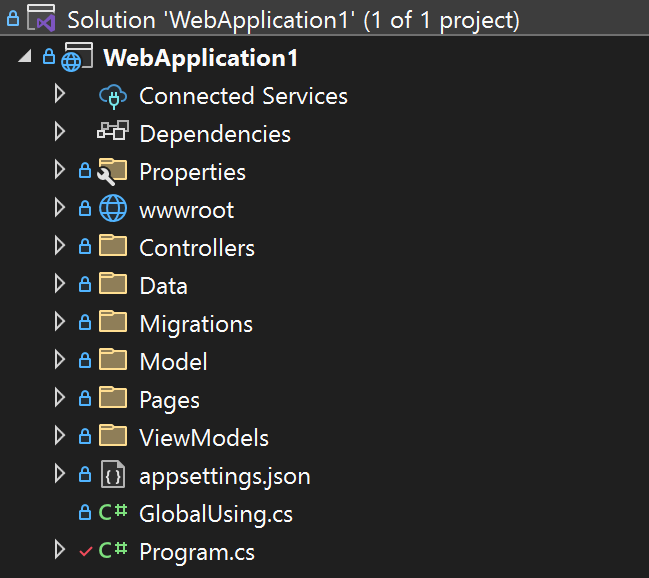
\includegraphics[height=220px]{img/solution-explorer-screenshot}
	\caption{Projekt struktúra}
	\label{fig:project-structure}
\end{figure}

\subsection{Architektúra leírása}
A .NET-es integrált frontend és backend fejlesztés hatalmas előnye a rendszerezettség, a szabályszerű kommunikáció az egyes rétegek között (illetve ezen rétegek helyes elkülönölése), és a rengeteg beépített segédfüggvény/konfiguráció/cshtml tag. Kiemelném még a modellek használatát is, amelyek egyszerűbb és biztonságosabb (például SQL injection elleni védelem) adatbázis kezelést biztosítanak.

Az egyes route-ok konfigurálása is meglehetősen letisztult ebben a keretrendszerben. A "Pages" mappa\footnote{A "Pages" mappa, ahogy a neve is mutatja, tartalmazza a weboldal egyes oldalait. Bővebb kifejtés a Frontend című fejezetben.} fájlstruktúrája alapján automatikusan létrejönnek a route-ok, ha a "Program.cs"-ben megadjuk a programnak, hogy hozza létre őket:

\lstset{caption={Route-ok konfigurálása}, label=src:routing}
\begin{lstlisting}[language={[Sharp]C}]
	app.UseRouting();
\end{lstlisting}

A frontend és a backend közötti hagyományos JavaScript segítségével történő kommunikáción kívül, a cshtml formátum miatt lehetőség nyílik egyszerűbb esetekre közvetlen kapcsolatot is létesíteni a backend és a frontend között. Például:

\lstset{caption={Frontend modell egy alkalmazása}, label=src:model}
\begin{lstlisting}[language={HTML}]
	<h1>Username</h1>
	<p>@Model.UserData.Username</p>
\end{lstlisting}

Itt ugye mint látható a modellből tudunk adatot lekérdezni.
De mi is a "Model" pontosan? Ugyebár az ASP .NET Web App keretrendszer úgy működik, hogy minden oldal (Razor page) egy .cshtml és egy .cs fájl együtteséből áll össze. A .cs kiterjesztésű fájl az adott oldal modellje. Itt definiálhatunk adatszerkezeteket és függvényeket, mint például az OnGet() és OnPost(), amelyek beépített (opcionális) metódusok, és ahogy a nevük is mutatja,
az oldalról érkező GET és POST requesteket kezelik. Tehát például,
ha az adott oldalon egy darab form-unk van, amit POST metódussal
be akarunk küldeni a szervernek, ezt JS (JavaScript) kód írása nélkül biztonságosan meg tudjuk tenni.

\section{Backend}

Először is nézzük meg az alkalmazás egyes backendet felépítő elemeit, és azok funkcionalitását, kezelését.

\subsection{appsettings.json}

Az appsettings.json egy konfigurációs
fájl. Ebben lehet alkalmazásszintű beállításokat tárolni, például:
adatbáziskapcsolati stringeket,
API kulcsokat,
logolási beállításokat,
vagy bármilyen egyedi, fejlesztő által definiált értéket.
Az értékeket a program könnyen kiolvassa a beépített konfigurációs
rendszer segítségével (pl. Configuration["Kulcs"] vagy
erősen típusos binding-gel). Ez segít elkülöníteni a kódot a
konfigurációtól, így könnyebb a karbantartás, környezetenkénti
eltérés kezelése (pl. fejlesztői vs. éles környezet).

\subsection{Program.cs}
Ez a fő program fájl. Ebben készítjük
elő a webalkalmazásunk tulajdonságait (persze a C\# egyszerűségének
hála ez nem sok plusz feladattal jár, csupán a helyes függvényeket
kell meghívni helyes sorrendben, attól függően, hogy hogyan
akarjuk konfigurálni az alkalmazást.) Itt lehet beállítani a
korábban említett routing-ot, az autentikációt, a cookie-kat,
a session-t, a fejlesztői és éles környezeteket, és még sok minden mást. Itt tudjuk felkonfigurálni a modellt, az adatbázist
és az oldalakat (Pages) is. ezután az app.Run() függvény hívással
tudjuk ténylegesen elindítani a weboldalt, és ekkor localhoston
el is kezd futni.

\subsection{Modellek}
Minden adatbázis táblának létrehozunk egy modellt
(bővebb kifejtés az "adatbázis" pontban). Ezek mind C\# osztályok
táblánként, és minden oszlop egy külön propertynek feleltethető meg.

\subsection{API}
Az ASP.NET-es struktúra úgy működik, hogy miután a 
Program.cs-ben felkonfiguráltuk a szükséges dolgokat, megalkottuk a modelleket, létrehoztuk a HTML lapokat, már csak
egy fontos dolog maradt hátra. A frontend-backend kommunikáció.
Említés esett már arról, hogy egyszerűbb esetekben ezt a HTML-ben
bizonyos tagekkel meg tudjuk tenni, de a nem triviális esetek
megoldására is egyszerű módot kinál a .NET. A Controllers
mappában minden modellnek (vagyis minden adatbázis táblának)
létrehozunk egy Controller fájlt is. Ebben fogunk API-végpontokat
definiálni, melyeket a frontenden JavaScript segítségével tudunk
meghívni, és ezáltal adatot közvetíteni a felhasználó és a szerver
között (oda-vissza). Az API-endpointok tesztelésére és leírására
egy hasznos, szintén beépített, megoldást használhatunk, a Swaggert.
Ezt is a Program.cs fájlban állíthatjuk be.\footnote{Szigorúan csak 
Development módban jelenjen meg, adatvédelmi/adat hitelességi okokból.}

\section{Frontend}
Térjünk át a frontend réteg alkotóelemeire, és ezek működésére. Itt is komponensenként fogom bemutatni a felhasznált technológiákat.

\subsection{Layout}
A "Pages" mappa tartalmazza az oldalakat. A keretrendszer ugyebár úgy működik, hogy minden oldal (Razor page) egy .cshtml és egy .cs
fájl együtteséből áll össze. A Pages mappa ezeket a párosokat tartalmazza, további kisebb mappákra bontva a funkció csoportok alapján. Az alább mellékelt ábrából (\ref{fig:pages-structure}. ábra) látható tehát, hogy például a bejelentkező felületet a következő linken tudjuk elérni: "localhost:<<port>>/Account/Login".

\begin{figure}[H]
	\centering
	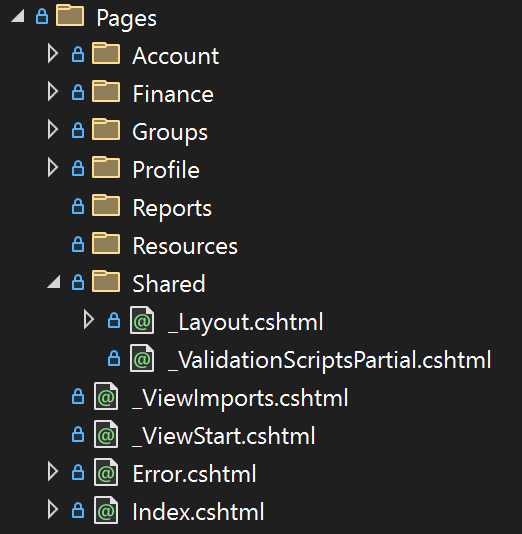
\includegraphics[height=240px]{img/solution-explorer-pages-screenshot}
	\caption{Pages struktúra}
	\label{fig:pages-structure}
\end{figure}

Találhatók még ebben a mappában egyéb segédfájlok is, mint például az Error.cshtml, ami az esetleges hibák esetén jelenik meg. Kiemelendő még a Shared mappa, amiben található egy Layout.cshtml fájl is (modell nélkül). Ez, ahogy a neve is mutatja egy alap sablont biztosít az alkalmazás felületének. A weboldal egy (a képernyő baloldán lévő) főmenüből, egy kis (az oldal tetején található) menüsávból, a fő tartalmi részből áll, illetve egy footer részből áll. A footer és a menüsávok kódját tartalmazza a Layout.cshtml között a tartalomnak "kihagyott" rész: 
\lstset{caption={Layout extension ASP.NET keretrendszerben}, label=src:csharp}
\begin{lstlisting}[language={HTML}]
	<div class="container-fluid">
	@RenderBody()
	</div>
\end{lstlisting}

A RenderBody() függvény (szintén beépített .NET metódus)
behelyezi az adott oldal HTML kódját ebbe a div HTML elembe. Ez
automatikusan megtörténik az összes oldal esetében amelyre
navigál a felhasználó. Ha valami miatt éppen nem ezt a sablont akarjuk követni egy oldalunkkal (például: Bejelentkező felület), akkor az adott oldal HTML kódjába beírhatjuk hogy ne sablont kövessen:

\begin{lstlisting}[language={[Sharp]C}]
	@{
		Layout = null; // Remove layout if you want a standalone page
	}
\end{lstlisting}

\subsection{static}
A "wwwroot" mappában található az összes statikus erőforrás (static resource). Itt a hagyományosan használt mappastruktúrát követtem az alkalmazás készítésekor, azaz létre lettek hozva a következő mappák:
\begin{itemize}
	\item "js": JavaScript kódok
	\item "css": CSS stylesheetek
	\item "img": Képek  
\end{itemize}
A frontend rész formázását Bootstrap keretrendszer felhasználásával valósítottam meg. Ezt úgy importáltam a projektbe, hogy a kész CSS/JS fileok vannak letöltve ugyanide, a wwwroot mappába, ezen kívül egy külső hivatkozás van egy betűtípusra. 

\section{Adatbázis}
Az alkalmazás adatbázisa egy localhoston futó MySQL adatbázis.
A MySQL-t sok szempont miatt szokták kisebb alkalmazásokhoz
használni, ezek közé tartozik például az a nem elhanyagolható
indok, hogy teljesen ingyenes a használata. Illetve szintén
az egyszerűségét tudnám kiemelni, és a kompatibilitását az ASP.NET keretrendszerrel. Egy darab adatbázis lett létrehozva, azon belül több tábla található, melyek természetesen kapcsolódnak egymáshoz. Az adatmodell a relációs adatbázisok normalizálási elvein alapul, és a harmadik normálformáig (3NF) került kialakításra.

\subsection{Backend - Adatbázis kapcsolat}
A backend és az adatbázis kapcsolata relatív egyszerűen megvalósítható az ASP.NET keretrendszerben.
A NuGet package managerből az EntityFramework egyes csomagjait,
illetve a MySQL Connector csomagot letöltve már alig van
dolgunk. Az appsettings.json fájlban tudjuk a connection
stringet definiálni.

\lstset{caption={Adatbázis Connection String}, label=src:connstring}
\begin{lstlisting}[language={HTML}]
	"ConnectionStrings": {
		"MySqlConnection": "server=localhost;port=3306;database=betterspend;user=root;password=<<password>>;"
	}
\end{lstlisting}

majd a Program.cs fájlban tudunk ténylegesen csatlakozni:

\lstset{caption={Program.cs: Adatbázis csatlakozás}, label=src:csharp}
\begin{lstlisting}[language={[Sharp]C}]
	// Get MySQL connection string from configuration
	string connectionString = builder.Configuration.GetConnectionString("MySqlConnection");
	
	// Add DB Context to the application
	builder.Services.AddDbContext<ApplicationDbContext>(options =>
	{
		options.UseMySql(connectionString, ServerVersion.AutoDetect(connectionString));
	});
\end{lstlisting}

A tényleges adatbázis modellje:

\lstset{caption={Adatbázis modell}, label=src:dbmodel}
\begin{lstlisting}[language={[Sharp]C}]
	using WebApplication1.Model;
	namespace WebApplication1.Data
	{
		public class ApplicationDbContext : DbContext
		{
			public ApplicationDbContext(DbContextOptions<ApplicationDbContext> options)
			: base(options)
			{
			}
			
			public DbSet<User> Users { get; set; }
			public DbSet<Transaction> Transactions { get; set; }
			public DbSet<Category> Categories { get; set; }
			
		}
	}
\end{lstlisting}

Ezután már az adatbázisunk össze van kötve teljesen az alkalmazással. ASP.NET-ben közvetlenül az adatbázishoz (lekérdezésekkel, parancsokkal) nem tudunk hozzáférni. Amihez hozzá tudunk férni azok a modell fájlok (pl. Model/User). Ezeket tudjuk módosítani LINQ segítségével egyszerűen, és ez szinkronizálni fogja
a tényleges adatbázisunkkal.

\subsection{Migrations}
A későbbi fejlesztések során migrációkat használhatunk az adatbázis verziókövetésére és a változtatások biztonságos, konzisztens bevezetésére. A migrációk használata Entity Framework Core segítségével történik, ahol a DbContext osztály definiálja az adatbázis szerkezetét. A módosításokat a dotnet ef migrations add paranccsal lehet rögzíteni, majd a dotnet ef database update parancs segítségével alkalmazni az adatbázisra. Ez lehetővé teszi a séma változásainak verziókövetését és biztonságos frissítését.



\section{Tesztek}
---

\section{UML diagramok}
---
